\documentclass[11pt,a4paper]{article}
\usepackage[margin=25mm]{geometry}
\usepackage{lmodern}
\usepackage[T1]{fontenc}
\usepackage{amsmath,amssymb,amsthm,booktabs,url,microtype,enumitem}
\usepackage{tikz}
\usetikzlibrary{arrows.meta,positioning}
\usepackage[hidelinks]{hyperref}

\newtheorem{theorem}{Theorem}
\newtheorem{lemma}{Lemma}
\theoremstyle{definition}
\newtheorem{definition}{Definition}
\theoremstyle{remark}
\newtheorem*{remark}{Remark}

\newcommand{\AS}{\mathrm{AS}}
\newcommand{\auth}{\mathsf{authorized}}
\newcommand{\Pp}{\mathsf{P}}      % Provider+
\newcommand{\nP}{\mathsf{nP}}     % Not Provider+
\newcommand{\nA}{\mathsf{nA}}     % No Attestation
\newcommand{\up}{\mathsf{up}}
\newcommand{\down}{\mathsf{down}}
\newcommand{\peer}{\mathsf{peer}}
\newcommand{\Valid}{\textup{\textsc{Valid}}}
\newcommand{\Invalid}{\textup{\textsc{Invalid}}}
\newcommand{\Unknown}{\textup{\textsc{Unknown}}}
\newcommand{\maxup}{\mathit{max\_up}}
\newcommand{\minup}{\mathit{min\_up}}
\newcommand{\maxdown}{\mathit{max\_down}}
\newcommand{\mindown}{\mathit{min\_down}}
\newcommand{\lead}{\mathrm{lead}}
\newcommand{\VF}{\mathrm{VF}}
\newcommand{\lean}[1]{\texttt{#1}}

\title{Securing Internet Routing:\\Machine-Checked Proofs for ASPA Route-Leak Detection\\and a False-Positive Flaw in the ASRA Extension}
\author{Nobuo Otoi\\BA Cybersecurity, Tokyo, Japan\\\texttt{otoi@ba-cybersecurity.com}}
\date{October 2026 (version 1)}

\begin{document}
\maketitle

\begin{abstract}
Route leaks---BGP announcements that send Internet traffic through networks that should not carry
it---have repeatedly caused large outages and traffic interception.
ASPA (Autonomous System Provider Authorization) lets BGP speakers detect route leaks by checking an
AS\_PATH against RPKI-signed lists of provider ASes. The verification procedure of
draft-ietf-sidrops-aspa-verification has reached working-group consensus, and its correctness
properties are stated in prose (Section~5.2 and Appendix~B of the draft).
We transcribe Sections~5.3--5.6 and prove in Lean~4, for paths of any length, assuming that business
relationships are seen consistently from both ends and that every registered ASPA lists exactly the
providers of its AS:
the procedure never marks a valley-free path \Invalid;
a \Valid{} outcome implies the path is valley-free;
Property~1 of Appendix~B holds;
and under full deployment the procedure never returns \Unknown, so that \Valid{} and \Invalid{} coincide
exactly with valley-free and route leak.
We then analyse ASRA (Autonomous System Relationship Authorization), a proposed extension that adds
fake-link detection and is stated to ``fully preserve the route leak detection capabilities of ASPA''.
Step~4 of its downstream enhancement, in both Algorithm~A and Algorithm~B, marks valley-free paths
\Invalid: when the origin has no ASPA and the apex of the path is a lateral-peer hop, a single AS with
correct ASPA and ASRA objects suffices. The smallest instance has four ASes, and in exhaustive
enumeration of four-AS topologies every false positive comes from Step~4.
Starting the Step~4 range at $\maxup+1$ instead of $\minup+1$ removes the flaw; we prove in Lean that
the modified step fires only on route leaks.
We also record a consequence of ASPA for AS-path poisoning.
Proofs and scripts are released as artifacts.
\end{abstract}

\noindent\textbf{Keywords:} network security; Internet routing security; BGP; route leaks; RPKI; ASPA; ASRA; formal verification; Lean~4; IETF standardization

\section{Introduction}

A route leak is a BGP announcement that violates the export policies implied by business
relationships, usually formalised by the valley-free model of Gao and Rexford~\cite{gao-rexford,rfc7908}.
ASPA~\cite{aspa-profile,aspa-verification} lets a customer AS publish, as an RPKI object, the set of its
provider ASes. From these objects a BGP speaker bounds the up-ramp and the down-ramp of a received
AS\_PATH; if the two ramps cannot meet, the route is a leak.

The draft states its guarantees in prose: the AS\_PATH is valid if the combined ramp lengths reach the
path length, and leaked or malformed otherwise (Section~5.2); Appendix~B lists detection properties
under partial deployment. An earlier formulation of the downstream algorithm was analysed by its
designers, who stated two theorems and proved them by enumeration for small cases with an induction
step to be described later~\cite{sriram-heitz}. The current formulation (Sections~5.4--5.6) has no
published proof. Because the procedure will run in router code across the Internet, and because
extensions are being designed on top of it, we give machine-checked arguments.

\paragraph{Contributions.}
\begin{enumerate}[nosep]
  \item A literal, executable transcription of Sections~5.3--5.6 of draft-ietf-sidrops-aspa-verification,
        cross-checked against a Gao--Rexford ground truth on all labelled topologies of up to four ASes,
        including non-transparent route servers (835{,}224 combinations of path, receiver and deployment
        set at $n=4$), and against all 25 rows of the worked examples referenced by the draft~\cite{aspa-examples}.
  \item Lean~4 proofs, for paths of any length, of no false positive, soundness of \Valid, Property~1 of
        Appendix~B, and exactness under full deployment (Section~\ref{sec:aspa}). The development uses core
        Lean only, contains no \lean{sorry}, and does not depend on \lean{Classical.choice}.
  \item A false-positive flaw in Step~4 of the ASRA downstream enhancement~\cite{asra}, with a four-AS
        counterexample (Section~\ref{sec:asra}).
  \item A modified Step~4 and a Lean proof that it fires only on route leaks (Section~\ref{sec:fix}).
  \item Two observations, on AS-path poisoning and on the transparent route-server exception
        (Section~\ref{sec:obs}).
\end{enumerate}

\section{ASPA verification}
\label{sec:aspa-bg}

Let the COMPRESSED\_AS\_PATH be $\AS(N),\dots,\AS(1)$, where $\AS(1)$ is the origin, $\AS(N)$ is the
neighbour of the verifying AS, and $\AS(N+1)$ is the verifying AS. Let $\mathrm{SPAS}(x)$ be the union of
the provider sets in the valid ASPAs of $x$, defined when $x$ has at least one valid ASPA. The provider
authorization function (Section~5.3) is
\[
  \auth(x,y)=
  \begin{cases}
    \nA & \text{if $x$ has no valid ASPA},\\
    \Pp & \text{if } y\in\mathrm{SPAS}(x),\\
    \nP & \text{otherwise}.
  \end{cases}
\]
Writing $a_i=\auth(\AS(i),\AS(i+1))$ and $b_j=\auth(\AS(j),\AS(j-1))$, the bounds of Section~5.4 are
\begin{align*}
  \maxup   &= \min\bigl(\{\, I\in[1,N-1] : a_I=\nP \,\}\cup\{N\}\bigr),\\
  \minup   &= \min\bigl(\{\, I\in[1,N-1] : a_I\neq\Pp \,\}\cup\{N\}\bigr),\\
  \maxdown &= N-J_{\nP}+1,\qquad \mindown = N-J_{\neq\Pp}+1,
\end{align*}
where $J_{\nP}=\max\{\,J\in[2,N] : b_J=\nP\,\}$ and $J_{\neq\Pp}=\max\{\,J\in[2,N] : b_J\neq\Pp\,\}$, and
$\maxdown=N$ (resp.\ $\mindown=N$) when the set is empty.
For a route received from a provider (downstream, Section~5.6), after the prerequisite steps 1--3,
\[
  \mathrm{out}_{\downarrow}=
  \begin{cases}
    \Invalid & \text{if } \maxup+\maxdown<N,\\
    \Unknown & \text{else if } \minup+\mindown<N,\\
    \Valid   & \text{otherwise.}
  \end{cases}
\]
For a route received from a customer, a lateral peer or a route server, and for a route received by a
route server (upstream, Section~5.5), the same rule applies with $\maxdown=\mindown=0$; we write
$\mathrm{out}_{\uparrow}$.

\section{Model}
\label{sec:model}

\paragraph{Hops.}
A path of $N$ ASes has $n=N-1$ hops. Hop $i$ ($0\le i<n$) goes from $\AS(i+1)$ to $\AS(i+2)$ and is the
triple $h_i=(\tau_i,\alpha_i,\beta_i)$, where $\tau_i\in\{\up,\down,\peer\}$ is its true type ($\up$: the
receiver is the sender's provider; $\down$: a customer; $\peer$: a lateral peer),
$\alpha_i=\auth(\AS(i+1),\AS(i+2))$ and $\beta_i=\auth(\AS(i+2),\AS(i+1))$.

\paragraph{Bounds as prefix lengths.}
For a predicate $P$ and a list $\ell$, let $\lead_P(\ell)$ be the length of the longest prefix of $\ell$
all of whose elements satisfy $P$, and let $\overleftarrow{h}=(h_{n-1},\dots,h_0)$. Then
\begin{align*}
  \maxup   &= 1+\lead_{\alpha\neq\nP}(h), & \minup   &= 1+\lead_{\alpha=\Pp}(h),\\
  \maxdown &= 1+\lead_{\beta\neq\nP}(\overleftarrow{h}), & \mindown &= 1+\lead_{\beta=\Pp}(\overleftarrow{h}).
\end{align*}
We checked by hand that these agree with the index-based definitions of Section~\ref{sec:aspa-bg},
including the empty-set cases; the literal Python transcription agrees with them on every enumerated
case; and both the Python transcription and the Lean definitions reproduce every row of the worked
examples~\cite{aspa-examples} (9 upstream, 10 downstream, 6 complex-relationship rows), on all reported
bounds and on the outcome. In Lean each row is checked by \lean{decide}.

\begin{definition}[Valley-free]
A sequence of hop types $\tau_0,\dots,\tau_{m-1}$ is \emph{valley-free}, written $\VF(\tau)$, if
\[
  \forall\, i<j<m:\quad \tau_i\neq\up\;\Longrightarrow\;\tau_j=\down ,
\]
that is, it matches $\up^{*}\,\peer^{?}\,\down^{*}$. The ground truth for a received route is $\VF$ of the
full sequence including the hop into the verifying AS, which is $\down$ for downstream verification and
$\up$ or $\peer$ for upstream verification.
\end{definition}

\begin{lemma}[\lean{vf\_snoc\_down}, \lean{vf\_snoc\_nondown}]
$\VF(\tau\cdot\down)\iff\VF(\tau)$, and for $t\neq\down$, $\VF(\tau\cdot t)\iff\forall i,\ \tau_i=\up$.
\end{lemma}

\paragraph{Assumptions.}
\begin{enumerate}[label=(A\arabic*),nosep]
  \item Consistency: $y$ is a provider of $x$ if and only if $x$ is a customer of $y$.
  \item ASPA correctness: if $x$ has a valid ASPA, then $y\in\mathrm{SPAS}(x)$ if and only if $y$ is a provider of $x$.
\end{enumerate}
From (A1) and (A2) every hop satisfies (Lean: \lean{hop\_correct})
\begin{equation}\label{eq:correct}
  \tau_i=\up\Rightarrow\alpha_i\neq\nP,\qquad
  \alpha_i=\Pp\Rightarrow\tau_i=\up,\qquad
  \tau_i=\down\Rightarrow\beta_i\neq\nP,\qquad
  \beta_i=\Pp\Rightarrow\tau_i=\down .
\end{equation}

\paragraph{Not modelled in Lean.}
Steps 1--3 of the procedures (empty path, neighbour-ASN check, AS\_SET) are assumed to have passed.
Route servers are covered only by the enumeration. Complex relationships are excluded by (A1). The
theorems do not require consecutive ASes to be neighbours, so they hold in particular for every real path.

\section{Machine-checked properties of ASPA}
\label{sec:aspa}

All results are in \lean{Aspa.lean} (Lean~4.33.1, core only, about 550 lines including the 25 example
checks). \lean{\#print axioms} reports at most \lean{propext} and \lean{Quot.sound} for every theorem.
Throughout, every hop satisfies~\eqref{eq:correct}.

\begin{theorem}[No false positive; \lean{down\_no\_false\_positive}, \lean{up\_no\_false\_positive}]
If $\VF(\tau)$ then $\mathrm{out}_{\downarrow}\neq\Invalid$. If $\tau_i=\up$ for all $i$, then
$\mathrm{out}_{\uparrow}\neq\Invalid$.
\end{theorem}
\begin{proof}[Proof sketch]
Let $k=\lead_{\alpha\neq\nP}(h)$. If $k=n$ then $\maxup=N$. Otherwise $\alpha_k=\nP$, so
$\tau_k\neq\up$ by~\eqref{eq:correct}, and $\VF(\tau)$ gives $\tau_j=\down$ for all $j>k$. Hence
$\beta_j\neq\nP$ for $j>k$, so $\maxdown\ge n-k$, and $\maxup+\maxdown\ge (k+1)+(n-k)=N$.
\end{proof}

\begin{theorem}[\Valid{} is sound; \lean{down\_valid\_sound}, \lean{up\_valid\_sound}]
If $\mathrm{out}_{\downarrow}=\Valid$ then $\VF(\tau)$. If $\mathrm{out}_{\uparrow}=\Valid$ then $\tau_i=\up$ for all $i$.
\end{theorem}
\begin{proof}[Proof sketch]
Let $k_1=\lead_{\alpha=\Pp}(h)$ and $k_2=\lead_{\beta=\Pp}(\overleftarrow{h})$. By~\eqref{eq:correct},
$\tau_i=\up$ for $i<k_1$ and $\tau_j=\down$ for $j\ge n-k_2$. \Valid{} gives $k_1+k_2\ge n-1$. If
$i<j$ and $\tau_i\neq\up$, then $i\ge k_1$, so $j\ge k_1+1\ge n-k_2$ and $\tau_j=\down$.
\end{proof}

\begin{theorem}[Appendix~B, Property~1; \lean{up\_property1}]
If some hop $i$ has $\tau_i\neq\up$ and $\alpha_i\neq\nA$ (its sender has an ASPA and sent the route
to a customer or a lateral peer), then $\mathrm{out}_{\uparrow}=\Invalid$, whatever the deployment status
of the other ASes.
\end{theorem}
\noindent This is Property~1 with ``AS~B doing ASPA'' read as AS~B running the upstream procedure; only
the ASPA of AS~A is needed.

\begin{theorem}[Full deployment; \lean{down\_full\_no\_unknown}, \lean{up\_full\_no\_unknown},\\ \lean{down\_full\_exact}]
If $\alpha_i\neq\nA$ and $\beta_i\neq\nA$ for all $i$, the outcome is never \Unknown. Consequently
$\mathrm{out}_{\downarrow}=\Valid\iff\VF(\tau)$ and $\mathrm{out}_{\downarrow}=\Invalid\iff\neg\VF(\tau)$.
\end{theorem}

\noindent\lean{aspa\_downstream} and \lean{aspa\_upstream} restate Theorems~1 and~2 for a topology and an
ASPA table satisfying (A1) and (A2), with the ground truth evaluated on the full hop sequence including the
hop into the verifying AS.

\section{A false positive in the ASRA downstream enhancement}
\label{sec:asra}

\subsection{The step}
draft-sriram-sidrops-asra-verification-05~\cite{asra} refines the downstream outcome using ASRA objects,
which list an AS's customers and lateral peers. In Algorithm~A, Step~2 returns early if $\minup=N$ or
$\minup+\mindown>N$, Step~3 checks for fake links, and Step~4 reads:
\begin{quote}\small
Else, if for any $i$ value from $(\minup+1)$ to $(N-\mindown)$, if $\AS(i)$ has ASPA and ASRA asserting
that $\AS(i+1)$ is a lateral peer (and not a Provider or Customer), then change the outcome to Invalid.
\end{quote}
Algorithm~B uses the range $(\minup+1)$ to $(N-1)$ and has no second early-exit condition. The draft
explains that Step~4 compensates for missing ASPA information about the next AS.

\subsection{Counterexample}
\begin{figure}[ht]
\centering
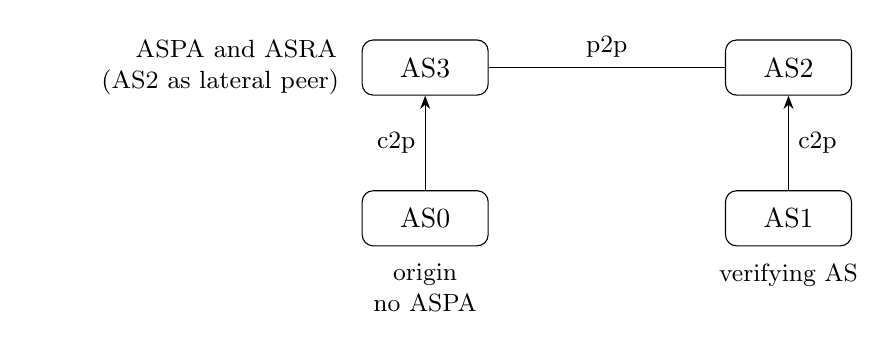
\begin{tikzpicture}[node distance=12mm and 30mm, as/.style={draw,rounded corners,minimum width=16mm,minimum height=7mm}]
  \node[as] (a3) {AS3};
  \node[as, right=of a3] (a2) {AS2};
  \node[as, below=of a3] (a0) {AS0};
  \node[as, below=of a2] (a1) {AS1};
  \draw[-{Stealth}] (a0) -- node[left,font=\small]{c2p} (a3);
  \draw (a3) -- node[above,font=\small]{p2p} (a2);
  \draw[-{Stealth}] (a1) -- node[right,font=\small]{c2p} (a2);
  \node[below=1mm of a0,font=\small,align=center]{origin\\no ASPA};
  \node[below=1mm of a1,font=\small,align=center]{verifying AS};
  \node[left=2mm of a3,font=\small,align=right,text width=38mm]{ASPA and ASRA\\(AS2 as lateral peer)};
\end{tikzpicture}
\caption{The four-AS counterexample. Arrows point from customer to provider.}
\label{fig:cex}
\end{figure}

In Figure~\ref{fig:cex}, AS1 receives from its provider AS2 the path with $\AS(1)=\text{AS0}$,
$\AS(2)=\text{AS3}$, $\AS(3)=\text{AS2}$ ($N=3$). Only AS3 registers objects: a correct ASPA (its providers,
which include neither AS0 nor AS2) and a correct ASRA listing AS2 as a lateral peer. The path is
valley-free ($\up$, $\peer$, then $\down$ into AS1). The bounds are
\begin{align*}
  \minup&=1 &&(\text{AS0 has no ASPA, so }\auth(\text{AS0},\text{AS3})=\nA),\\
  \maxup&=2 &&(\auth(\text{AS3},\text{AS2})=\nP),\\
  \mindown&=1 &&(\text{AS2 has no ASPA, so }\auth(\text{AS2},\text{AS3})=\nA),\\
  \maxdown&=2 &&(\auth(\text{AS3},\text{AS2})=\nP),
\end{align*}
so $\maxup+\maxdown=4\ge N$ and $\minup+\mindown=2<N$: ASPA alone yields \Unknown. In both algorithms,
Step~2 does not exit ($1\neq3$ and $1+1\not>3$); Step~3 detects no fake link (AS0 has no ASPA, and AS3's
ASRA lists AS2); Step~4 examines $i=2$, where $\AS(2)=\text{AS3}$ asserts that $\AS(3)=\text{AS2}$ is a
lateral peer, and returns \Invalid.

\paragraph{Cause.}
$\minup$ stops at AS0 only because AS0 has no ASPA. The true up-ramp continues to AS3, the legitimate apex.
Treating a lateral hop beyond $\minup$ as a leak is justified only once the up-ramp is known to have ended,
that is, at an $\nP$ pair. The configuration is common under partial deployment (a stub origin without
ASPA, its early-adopting transit provider peering laterally, a customer cone below the peer), and a single
adopting AS suffices.

\paragraph{Verification.}
We re-derived the counterexample from the specification text as above, for both algorithms. In Lean,
\lean{cex\_valley\_free}, \lean{cex\_aspa\_unknown} and \lean{cex\_step4\_fires} establish, by kernel
evaluation and without axioms, that the path is valley-free, that ASPA alone yields \Unknown, and that the
Step~4 condition holds over Algorithm~B's range. Algorithm~A's range is a sub-range
($N-\mindown\le N-1$) and contains $i=2$ here. Steps~2--3 are not modelled in Lean; that they pass is the
hand derivation above, confirmed by the Python model. Exhaustively, over all labelled four-AS topologies,
all simple paths received from a provider and all subsets of ASPA and ASRA adopters (ASRA adopters also
have an ASPA; all objects correct), each algorithm yields 4{,}608 labelled false-positive cases, all from
Step~4; Step~3 yields none, as expected, since with correct registrations every real link appears in an
ASPA, an ASRA-C or an ASRA-LP.

\subsection{A modified Step 4}
\label{sec:fix}
We propose to start the Step~4 range at $\maxup+1$ instead of $\minup+1$.

\begin{theorem}[\lean{step4\_fixed\_sound}]
Assume every hop satisfies~\eqref{eq:correct} and every asserted lateral peer is a true lateral peer
(\lean{LatCorrect}). If the modified Step~4 fires, then $\neg\VF(\tau)$.
\end{theorem}
\begin{proof}[Proof sketch]
Let $k=\lead_{\alpha\neq\nP}(h)$, so $\maxup=k+1$, and suppose the step fires at hop $i$ with $i>k$ and
$\tau_i=\peer$. Then $\alpha_k=\nP$, hence $\tau_k\neq\up$, and $\VF$ would force $\tau_i=\down$.
\end{proof}
\noindent The theorem is proved for Algorithm~B's range and hence holds for Algorithm~A's sub-range.
ASRA correctness enters only as the assumption \lean{LatCorrect}; we do not derive it from an ASRA table.

On the same enumeration the modified step has no false positives and still flags 6{,}144 leaks that ASPA
alone does not mark \Invalid; the original Step~4 flags 15{,}360. Every one of the 9{,}216 cases no longer
flagged has the same shape: the lateral hop is the first $\nP$ pair and the hop before it is $\nA$. There the
registered objects cannot distinguish a leak from the valley-free path of Figure~\ref{fig:cex}, so flagging
such cases necessarily produces false positives as well. We do not propose extending the up-ramp with the
receiver's ASRA-C: Section~4.1 of the ASRA draft excludes that direction, since a forged ASRA-C would let a
leaker evade detection.

\subsection{Editorial}
ASRA-05 cites Sections~5.1 (COMPRESSED\_AS\_PATH), 5.3 (ramp parameters), 5.4 (upstream) and 5.5
(downstream) of the ASPA verification draft; in revisions -28 and -29 these are Sections~5.2, 5.4, 5.5
and~5.6.

\section{Further observations}
\label{sec:obs}

\paragraph{AS-path poisoning.}
Suppose an origin $O$ with an ASPA announces the poisoned path $[O,X,O]$. Since $\auth(O,X)=\nP$, every AS
that verifies the path computes \Invalid: $O$'s providers (upstream) and also ASes further downstream, for
example a customer of $P$ receiving $[O,X,O,P]$. The only exception in our model is when $X$ is one of
$O$'s registered providers and has no ASPA itself, giving \Unknown; if $O$ has no ASPA the outcome is
\Unknown. Thus an ASPA-registered origin cannot poison arbitrary ASes. The draft does not state this
consequence, and in the SIDROPS archive (7{,}290 messages as of 2026-10-28, searched through the IETF
IMAP service) poisoning is mentioned only in passing and in other contexts. Since poisoning is used in
measurement and traffic engineering, a sentence in the deployment considerations may be useful.

\paragraph{Transparent route-server exception.}
Section~5.1 of the draft notes both that a leaker may strip its own ASN and that routes from a transparent
IX route server are a standard exception to the neighbour-ASN check. Together, a client that strips its
own ASN and re-announces a provider-learned route through a transparent route server reaches other
clients with a \Valid{} outcome. This requires deliberate path manipulation; the ASRA-TIX registrations
proposed in Section~3 of ASRA-05 target this case.

\section{Related work}
Sriram and Heitz~\cite{sriram-heitz} found that the downstream algorithm of revision -06 misclassified
some valid paths as unknown, proposed a corrected algorithm based on a $(K,L)$ ramp representation, and
stated two theorems characterising the three outcomes, proved by enumeration for small cases with an
induction step to be described later. Their formulation precedes the current max/min formulation; our
proofs are mechanised, cover the current text, and also cover upstream verification and Appendix~B.
The SIDROPS list and draft-geng-sidrops-aspa-analysis~\cite{geng} discuss ASPA's limitations informally,
and Farina et al.\ applied ASPA verification to collected BGP data~\cite{first-look}. Route-leak detection and
mitigation were defined in RFC~7908~\cite{rfc7908} and~\cite{route-leak-dm}, and BGP Roles with the OTC
attribute in RFC~9234~\cite{rfc9234}. On the formal-methods side, routing algebras~\cite{sobrinho,metarouting},
the FSR toolkit~\cite{fsr} and a mechanised convergence proof for policy-rich distance-vector
protocols~\cite{daggitt} address convergence and policy safety rather than the ASPA procedure. To our
knowledge no mechanised proof of ASPA's verification properties has been published. A search of the
SIDROPS archive (all messages mentioning both ASRA and lateral peers, and all messages since June 2026
mentioning ASRA or false positives) found no report of the ASRA Step~4 issue.

\section{Limitations}
The ground truth is the standard valley-free model; complex relationships, sibling ASes and per-prefix
policies are excluded. Route servers are verified only by bounded enumeration. The correspondence between
the draft's prose and our definitions is checked by hand, by testing and against all 25 rows of the
worked examples, but it is not proved. ASRA is an individual draft and may change; our analysis refers to
revision -05 as published on 2026-07-06. Datatracker states were checked on 2026-10-28
(ASPA verification: ``WG Consensus: Waiting for Write-Up'').

\section*{Artifacts}
\lean{lean/Aspa.lean} (Lean~4 v4.33.1, core only; \lean{lean Aspa.lean} prints only the
\lean{\#print axioms} lines) and \lean{model/} (Python~3: literal transcriptions \lean{model.py},
\lean{asra.py}; checkers \lean{check.py}, \lean{check\_asra.py}, \lean{fixcheck.py}, \lean{lost.py},
\lean{examples.py}).
Repository: \url{https://github.com/otoinobuo/aspa-verify}. Archived with this paper at \url{https://doi.org/10.5281/zenodo.23734450}.

\section*{Acknowledgements}
AI tools produced the proofs, code and text under the author's direction; the author chose the questions
and claims and checked all results.

\begin{thebibliography}{99}\small
\bibitem{aspa-verification} A.~Azimov, E.~Bogomazov, R.~Bush, K.~Patel, J.~Snijders, K.~Sriram,
  ``BGP AS\_PATH Verification Based on Autonomous System Provider Authorization (ASPA) Objects'',
  draft-ietf-sidrops-aspa-verification-29, October 2026.
\bibitem{aspa-profile} A.~Azimov et al., ``A Profile for Autonomous System Provider Authorization'',
  draft-ietf-sidrops-aspa-profile.
\bibitem{aspa-examples} K.~Sriram, O.~Borchert, M.~Matejka, ``ASPA-based AS path verification examples'',
  October 2026, \url{https://github.com/ksriram25/IETF/blob/main/ASPA_path_verification_examples.pdf}.
\bibitem{sriram-heitz} K.~Sriram, J.~Heitz, ``Insights into the accuracy of algorithms for ASPA based route
  leak detection'', SIDROPS WG, IETF~110, March 2021,
  \url{https://github.com/ksriram25/IETF/blob/main/ASPA-alg-accuracy-v2.pdf}.
\bibitem{asra} K.~Sriram et al., ``Autonomous System Relationship Authorization (ASRA) as an Extension to
  ASPA for Enhanced AS Path Verification'', draft-sriram-sidrops-asra-verification-05, July 2026.
\bibitem{geng} N.~Geng et al., ``An Analysis of ASPA-based AS\_PATH Verification'',
  draft-geng-sidrops-aspa-analysis-05, August 2026.
\bibitem{first-look} M.~Farina, M.~Trevisan, A.~Bartoli, ``A First Look at ASPA: Deployment, Route Leaks, and AS
  Relationships'', ACM Internet Measurement Conference (IMC), 2026, doi:10.1145/3777912.3839812.
\bibitem{rfc7908} K.~Sriram, D.~Montgomery, D.~McPherson, E.~Osterweil, B.~Dickson, ``Problem Definition and
  Classification of BGP Route Leaks'', RFC~7908, 2016.
\bibitem{rfc9234} A.~Azimov, E.~Bogomazov, R.~Bush, K.~Patel, K.~Sriram, ``Route Leak Prevention and Detection
  Using Roles in UPDATE and OPEN Messages'', RFC~9234, 2022.
\bibitem{route-leak-dm} K.~Sriram et al., ``Methods for Detection and Mitigation of BGP Route Leaks'',
  draft-ietf-idr-route-leak-detection-mitigation.
\bibitem{gao-rexford} L.~Gao, J.~Rexford, ``Stable Internet routing without global coordination'',
  IEEE/ACM Transactions on Networking 9(6), 2001, doi:10.1109/90.974523.
\bibitem{sobrinho} J.~L.~Sobrinho, ``An algebraic theory of dynamic network routing'', IEEE/ACM
  Transactions on Networking 13(5), 2005, doi:10.1109/TNET.2005.857111.
\bibitem{metarouting} T.~G.~Griffin, J.~L.~Sobrinho, ``Metarouting'', ACM SIGCOMM, 2005, doi:10.1145/1090191.1080094.
\bibitem{fsr} A.~Wang, L.~Jia, W.~Zhou, Y.~Ren, B.~T.~Loo, J.~Rexford, V.~Nigam, A.~Scedrov, C.~Talcott,
  ``FSR: Formal Analysis and Implementation Toolkit for Safe Interdomain Routing'', IEEE/ACM Transactions
  on Networking 20(6), 2012, doi:10.1109/TNET.2012.2187924.
\bibitem{daggitt} M.~L.~Daggitt, A.~J.~T.~Gurney, T.~G.~Griffin, ``Asynchronous convergence of policy-rich
  distributed Bellman-Ford routing protocols'', ACM SIGCOMM, 2018, doi:10.1145/3230543.3230561.
\end{thebibliography}
\end{document}
